\chapter{评审与结对编程} % Introduction chapter suppressed from the table of contents

客户：我们的客户以银行为主，他们很注重质量，所以一直很注重评审。他们对需求评审、代码走查等也很赞同，也能找到缺陷，对提升质量有作用。但他们最困惑的是通过设计评审很难发现缺陷。\\
我：你听说过敏捷的结对编程吗？\\
客户：听过，也给客户做过培训，但是一般管理层都接受不了用两个人干一个人的活，所以几乎都没有团队在实际工作中使用。\\
我：单做培训确实难以推动并持续，必须按3步走，按部就班才有效果，让我分享一下。

\hypertarget{ux80ccux666f}{%
\subsection{背景}\label{ux80ccux666f}}

\hypertarget{ux6708}{%
\subsubsection{4月}\label{ux6708}}

现场结对编程培训之前8个月，首次见这家客户的总监。他们想用一年时间改进软件开发质量。事后知道原来他们有个超过12月的大型项目，因为验收时质量不达标，不能通过风险的验收测试，被拒收。因为公司是老字号，不想影响声誉，请求客户给机会让他们重头再做，客户同意但估计产生的损失超过100万，所以高层下定决心必须改进软件质量，避免类似情况再发生。

\hypertarget{ux6708-1}{%
\subsubsection{7月}\label{ux6708-1}}

与客户签了CMMI服务合同后首先做差距分析， 首先收集各领导的关注点。\\
某部门经理最担心的是系统维护：如果有人员离职，新人要花很长时间才能上手。\\
技术总监更担心是有些交付后的缺陷会很花工作量：如某系统交付后开始使用的时候很正常，但过了9个月，用户量和数据量都增加了，偶尔会出现有些报表出错，我们架构师、工程师等，花了3个半月才发现其中某接口的参数有问题。\\
另外发现开发人员水平参差，也没有做好单元测试和代码评审，代码可读性低，其他程序员难以理解，在分析后的汇报里，建议利用TDD和面向对象的设计原则改善编码规范，并加强培训，推行结对编程培训，提高代码的可读性，方便日后维护。\\
最后发现很多项目资源不足，没有充分的时间确保代码的质量。

\textbf{给管理层汇报}\\
因缺陷绝大部分都是后期测试才发现、缺陷修改的总工作量很大（估计占项目总工作量30\%），建议加强开发单元测试。\\
因代码都是个别程序员负责，建议团队用结对编程，除了能提高质量也防止一人离开其他人无法跟进的风险。\\
也预警管理层开始时要预留15-25\%时间给开发团队，当后面返工量减少，以后的总工作量会降低（生产率提升）。\\

\hypertarget{ux5929ux57f9ux8badux8bfe}{%
\subsection{2天培训课}\label{ux5929ux57f9ux8badux8bfe}}

第一天讲面向对象设计原理，设计模式，测试驱动开发；\\
第二天讲结对编程：

\framebox{%
\begin{minipage}[t]{0.97\columnwidth}\raggedright

%\href{文件:Interview_Parnas_Screenshot_2025-01-21_162541.jpg}{400px}

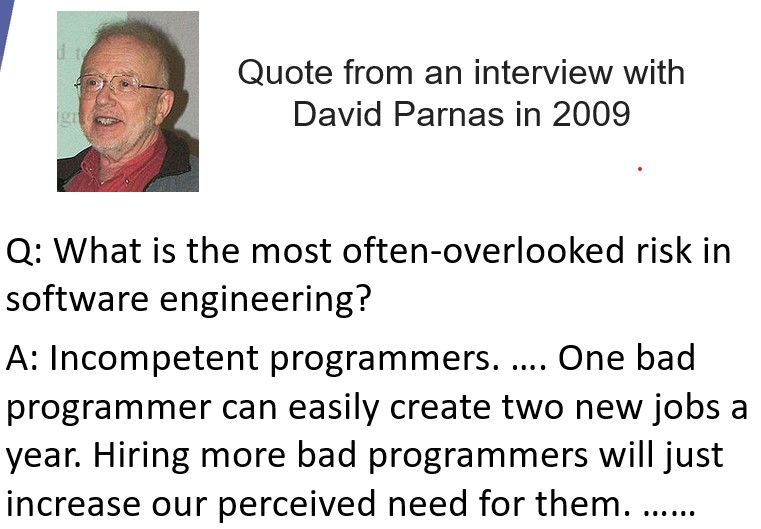
\includegraphics[width=10cm]{Interview_Parnas_Screenshot_2025-01-21_162541.jpg}

问：在软件工程常被忽略的最大风险是什么？

答：不称职的开发人员。据估计，美国需要的程序员数量超过20万。这完全是误导。这不是数量问题。我们有质量问题：一位糟糕的程序员一年内便很容易就会产生两个新岗位（的工作量）。如果我们有更多优秀的程序员，并且能够轻松识别他们，我们需要的就会减少，而不是增多。
\strut
\end{minipage}}

``也有人说：``卓越的程序员比优秀的程序员，不仅是好一些，而是倍数级的差异。''\\
请问你们觉得团队里程序员的水平也存在很大的差异？''\\
培训开始，对应以上幻灯片，我问大家。

你们是否觉得：

\begin{itemize}
\tightlist
\item
  交付后的软件难以维护
\item
  其他人难以读懂其他人的代码，员工离职后其他成员难以跟进和维护
\item
  代码总体设计不好，如缺乏良好架构，不灵活
\item
  系统交付后，有些缺陷需要很长时间才能修复好
\end{itemize}

如大家希望提高代码质量，必须从人入手。

如果你们团队也有同样问题，有什么好的解决办法呢？培训？\\
编码的最佳学习方式并非读书，而是动手做，所以单靠搞内部培训效果有限。有什么好方法帮助开发人员提升？

\hypertarget{ux4ee3ux7801ux8bc4ux5ba1}{%
\subsection{代码评审}\label{ux4ee3ux7801ux8bc4ux5ba1}}

就算评审规范做得很好能帮助初级程序员提升吗？
很难，因为代码都已经写完了。\\
比如我跟另一位老师看团队的代码，他们都写了起码几千行。我们的结论就是：虽然代码的设计很有问题，但已经到了这个地步，除非重写，否则单靠修正部分代码并没有帮助。这也是代码评审常常难以做好的主要原因。而且大家都要面子，如果在评审里，直接说他设计有问题，也可能会影响到大家的关系，所以在设计评审时难以找出缺陷，这很正常。\\
团队主管看程序员代码
只能把关防止严重错误，对程序员提升没有作用，所以评审不能有效保证代码质量，也不能帮助团队能力提升。\\
当写完了几千行代码后，就很难在评审时要求开发改动。程序员会觉得又不是不对，测试也跑得通，为什么要改。所以代码的质量问题应在写的时候就避免，这是结对编程的原理。你可以把结对编程看成是提高团队之间互相交流的培训方法。因为结对编程是在编码时针对具体问题集思广益进行解决，很容易落地，效果会比培训或评审好。\\
两个人互相讨论写代码才就是有效的培训，不能单挑单靠设计和编码规范和指南。

\hypertarget{ux57f9ux8badux8bbeux8ba1}{%
\subsection{培训设计}\label{ux57f9ux8badux8bbeux8ba1}}

有些人误以为：

\begin{itemize}
\tightlist
\item
  结对编程必须要找一位合适的搭档，人与人之间是否合得来最重要
\item
  结对时只是在旁边看
\item
  以为仅仅是教同伴应怎么做
\item
  以为只是看，作为人手编译器，只看代码是否写对，能否通过编译
\end{itemize}

我们针对这些重点设计一天培训。

\hypertarget{ux57f9ux8badux91cdux70b9}{%
\subsection{培训重点}\label{ux57f9ux8badux91cdux70b9}}

要培训有效，必须利用练习，让学员动手动脑筋。

\framebox{%
\begin{minipage}[t]{0.97\columnwidth}\raggedright
结对编程和实践说明

练习\#1和讨论：代码阅读\\
结对编程说明\\
练习\#2和讨论：设计和结对编程\\
练习\#3和讨论：Code Review和Pair Programming\\
练习\#4 怎样开始结对编程：10分钟结对编程\\
讨论：10分钟正确结对编程\\
练习\#5：队伍结对编程\\
Pair-Solo Programming\\
\strut
\end{minipage}}

练习一：用10条代码实例，每一条分A与B两种方式写，问学员那种更容易读懂，说明代码应怎样写才能让一般人容易读懂\\
练习二：先自己按面向对象做总体设计
然后两人结对分享设计做出最终设计学员讨论结对是否有效\\
然后解释若要持久，必须轮流替换伙伴，也介绍各类结对方式的利弊，例如：

\begin{description}
\tightlist
\item[]
Public-private pair programming ; pair - solo programming
\end{description}

练习四：先2人试试结对\\
练习五：六人为一队，轮流合作写程序，让学生体验交换。（详见附件）\\

\hypertarget{ux7ecfux9a8cux5206ux4eab}{%
\subsection{经验分享}\label{ux7ecfux9a8cux5206ux4eab}}

结对编程需要2人对话沟通，例如某人写代码时，另外一个人提问题，有些不习惯编写代码边说话沟通，培训时，预先写好台词。如果想多了解结对编程如何沟通，可参考书的实例。\\
有些程序员比较内向，不想说话，我们会用角色扮演：
先写好台词，让他们展示在结对编程时如何沟通。
帮助他们先打出一步，鼓励尝试。\\
注：如果想了解结对编程如何沟通，可以参照Robert
MARTIN先生的保龄球游戏实例（参考书里第6章），了解两个人如何从需求、总体类设计、按TDD写单元测试用例、然后写代码，让它通过，一步一步最终完成整个程序。\\

\hypertarget{ux603bux7ed3}{%
\subsection{总结}\label{ux603bux7ed3}}

培训开始时用例子说明结对编程除了能帮助团队知识分享和提高团队精神以外，更能：\\
*提高代码质量和可读性（编码规范）

\begin{itemize}
\tightlist
\item
  提高代码复用
\item
  加强测试驱动开发\\
\end{itemize}

利用互动练习让学员亲身体验结对编程的原则：

\begin{enumerate}
\tightlist
\item
  一边写代码一边说
\item
  提问，如：这方法是否归为这个类
\item
  每人带纸和笔（最好铅笔）
\item
  不断想复用
\end{enumerate}

\begin{description}
\item[]
\begin{description}
\tightlist
\item[]
-\/-\/- *** === *** -\/-\/-\\
\end{description}
\end{description}

客户：我猜你说的3步是：\\
第一步，高层认同软件质量问题的严重性，为此交过学费，知道损失多大\\
第二步，管理层不仅了解软件的质量问题和改善措施，更需要内部立项做培训和投入资源（人力），做过程改进\\
第三步才是具体的培训课。因为缺乏第一步和第二步，所以之前做完了结对编程培训后，没有效果\\
我：厉害，完全对。结对编程只是改进的一种方法，如果高层不关注、不立项、不投入资源，不会有改进效果。\\
结对编程这方法在70年代已经开始，与TDD、代码重构已经都经过验证能有效改善质量减少返工。所以结对编程本身没问题，要解决的问题是总体质量改进。\\
若要成功推行结对编程，必须先说服管理层，投入时间和资源，但投资会有好回报。\\
结对只是一种有效的改进方法，团队必须有每个迭代回顾，持续提升的好习惯，不可能单靠管理层下命令来推行，更好是团队自己有改进的动力，选择使用结对编程来提升质量，减少返工。

\textbf{本章最佳实践对应}：

\begin{itemize}
\tightlist
\item
  CMMI

  \begin{itemize}
  \tightlist
  \item
    单元测试：PR 2.X 3.X 所有实践
  \end{itemize}
\item
  XP

  \begin{itemize}
  \tightlist
  \item
    结对编程，代码共同拥有 都是XP里的实践
  \end{itemize}
\end{itemize}

\hypertarget{ux9644ux4ef6}{%
\section{附件}\label{ux9644ux4ef6}}

\hypertarget{ex-5}{%
\subsection{Ex 5}\label{ex-5}}

%Screenshotfrom2025-02-1620-57-07.png


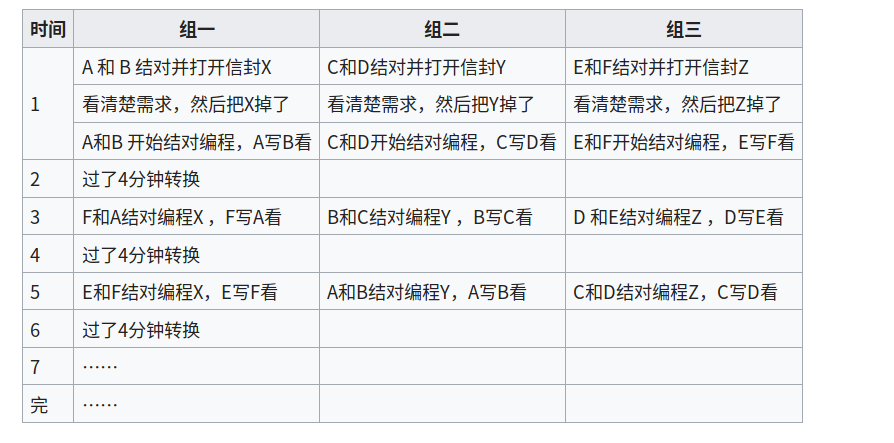
\includegraphics[width=10cm]{Screenshotfrom2025-02-1620-57-07.png}




